\section{Gate driver} \label{section:gatedriver}

\subsection{What is a gate driver}
A \textit{gate driver} is an IC which applies logic to and amplifies its inputs. This allows for for example an MCU or other low powered circuits to drive MOSFETS at frequencies above 1kHz. In addition to this a gate driver allows the switching of a high side MOSFET in a half bridge which cannot be done without a gate driver and additional components. Depending on the driver a multitude of safety features can be used, such as the prevention of enabling both MOSFETS in a half bridge as this would cause a short-circuit.

\subsection{Hardware}
Our design will be using the IRS2004(S)PBF gate driver from Infineon \cite{IRS2004PBF_Datasheet}. This driver was chosen as it is available in a PDIP and SOIC package which allows for breadboard testing and PCB design without changing chips. The IRS2004 has two inputs IN and SD, the IN pin is used to select the active MOSFET, HIGH or LOW. The SD pin allows for PWM-control and disabling of the chip, this is achieved by disabling the outputs if LOW and enabling them if HIGH.

Due to the single input IN to select the active MOSFET it is impossible to activate both MOSFETS simultaneously due to an internal dead time which makes sure one MOSFET is disabled before the other is enabled.

\subsubsection{High side MOSFET}
To drive the HIGH side MOSFET of a half bridge a bootstrap capacitor and diode are required. These are required as the MOSFET needs a positive voltage across its gate and source pins. This is a problem as when the MOSFET is conducting the source voltage is equal to the drain voltage. This means a greater voltage than the drain voltage is required to drive the MOSFET. In our design the drain voltage equals the input voltage which is 24V while the gate drive operates on 12V. As such the gate to source voltage van never be positive when the MOSFET is conducting, as a result the MOSFET will turn off and stop conducting.

To overcome this problem a bootstrap capacitor is used to increase the gate to source voltage to the source voltage plus the gate driver supply voltage. This capacitor needs to be charged to function, it is therefore important to switch the MOSFET at 100kHz or more. To charge the bootstrap capacitor a diode is used. Both of these components are external and can thus be chosen as necessary. \autoref{fig:GateDriverConnection} displays a typical connection of a gate driver. The bootstrap diode and capacitor are connected to the Vb pin of the gate driver. In total there will be three of such circuits within our final PCB design.

\begin{figure}[H]
    \centering
    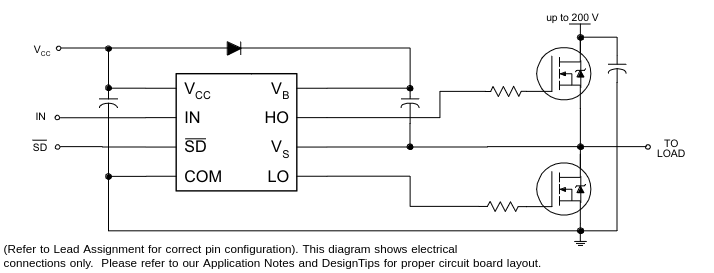
\includegraphics[width=0.5\textwidth]{img/GateDriver/Typical Connection Gate Driver.png}
    \caption{Typical Connection Gate Driver}
    \label{fig:GateDriverConnection}
\end{figure}

\subsection{Software}




% \begin{lstlisting}[caption={Start 3 PMW signals on timer 2 and mamage duty cycle},label={lst:STMSetup},language=C]
%     /* Initialize all configured peripherals */
%     MX_GPIO_Init();
%     MX_TIM2_Init();
%     MX_ADC1_Init();
%     MX_TIM1_Init();
%     MX_TIM3_Init();
%     /* USER CODE BEGIN 2 */

%     // Start PWM generation on three channels on timer 2
%     HAL_TIM_PWM_Start(&htim2, TIM_CHANNEL_1);
%     HAL_TIM_PWM_Start(&htim2, TIM_CHANNEL_2);
%     HAL_TIM_PWM_Start(&htim2, TIM_CHANNEL_3);

%     // If two timers are needed uncomment these
%     // HAL_TIM_PWM_Start(&htim3, TIM_CHANNEL_1);
%     // HAL_TIM_PWM_Start(&htim3, TIM_CHANNEL_2);
%     // HAL_TIM_PWM_Start(&htim3, TIM_CHANNEL_3);
%     // HAL_TIM_PWM_Start(&htim1, TIM_CHANNEL_1);
    
%     // Startup sequence
%     // Set active MOSFETS
%     HAL_GPIO_WritePin(GPIOC, GPIO_PIN_13, HAL_GPIO_ReadPin(GPIOB, GPIO_PIN_7)); // Set output U to HAL state W
%     HAL_GPIO_WritePin(GPIOC, GPIO_PIN_14, HAL_GPIO_ReadPin(GPIOB, GPIO_PIN_5)); // Set output V to HAL state U
%     HAL_GPIO_WritePin(GPIOC, GPIO_PIN_15, HAL_GPIO_ReadPin(GPIOB, GPIO_PIN_6)); // Set output W to HAL state V

%     // OR

%     GPIOC->ODR |= GPIOB->IDR << 8;;
    
%     /* USER CODE END 2 */
    
%     /* Infinite loop */
%     /* USER CODE BEGIN WHILE */
%     while (1)
%     {
    
%         HAL_ADC_Start(&hadc1);
%         HAL_ADC_PollForConversion(&hadc1, HAL_MAX_DELAY);
%         PWMPulse = HAL_ADC_GetValue(&hadc1) / 20;
    
%         /* USER CODE END WHILE */
    
%         /* USER CODE BEGIN 3 */
%     }
%     /* USER CODE END 3 */
% \end{lstlisting}

% See code \autoref{lst:STMSetup}.

% \begin{lstlisting}[caption={Read HAL ADC for PWM duty cycle control},label={lst:HalADC},language=C]
%     HAL_ADC_Start(&hadc1);
%     HAL_ADC_PollForConversion(&hadc1, HAL_MAX_DELAY);
%     PWMPulse = HAL_ADC_GetValue(&hadc1) / 20;
% \end{lstlisting}
% See code \autoref{lst:HalADC}.

% \begin{lstlisting}[caption={Interrupt routine using Hall sensor data},label={lst:stm32f4xx_it},language=C]
%     void EXTI9_5_IRQHandler(void)
%     {
%       /* USER CODE BEGIN EXTI9_5_IRQn 0 */
    
%     	//TIM2->CCR3 = HAL_GPIO_ReadPin(GPIOB, GPIO_PIN_5) * PWMPulse;
    
%     	// Save current state of Timers with new PWM duty cycle
%     	int PWMU = PWMPulse * CheckActive(TIM2->CCR1);
%     	int PWMV = PWMPulse * CheckActive(TIM2->CCR2);
%     	int PWMW = PWMPulse * CheckActive(TIM2->CCR3);
    
%     	// Set PWM duty cycle to zero for switching MOSFETS states
%     	TIM2->CCR1 = 0;
%     	TIM2->CCR2 = 0;
%     	TIM2->CCR3 = 0;
    
%     	// Set new MOSFETS states
%     	HAL_GPIO_WritePin(GPIOC, GPIO_PIN_13, HALPrevW); // Set output U to HAL state W
%     	HAL_GPIO_WritePin(GPIOC, GPIO_PIN_14, HALPrevU); // Set output V to HAL state U
%     	HAL_GPIO_WritePin(GPIOC, GPIO_PIN_15, HALPrevV); // Set output W to HAL state V
    
%     	HALPrevU = HAL_GPIO_ReadPin(GPIOB, GPIO_PIN_5);
%     	HALPrevV = HAL_GPIO_ReadPin(GPIOB, GPIO_PIN_6);
%     	HALPrevW = HAL_GPIO_ReadPin(GPIOB, GPIO_PIN_7);
    
%     	// OR
    
%     	GPIOC->ODR |= HALPrev;
%     	HALPrev = GPIOB->IDR << 8;
    
%     	// Set PWM duty cycle to previous saved state of preceding channel
%     	TIM2->CCR1 = PWMV;
%     	TIM2->CCR2 = PWMW;
%     	TIM2->CCR3 = PWMU;
    
%     	// Cycle through states
%     	/*int temp   = PWMPulse * CheckActive(TIM2->CCR1);
%     	TIM2->CCR1 = PWMPulse * CheckActive(TIM2->CCR2);
%     	TIM2->CCR2 = PWMPulse * CheckActive(TIM2->CCR3);
%     	TIM2->CCR3 = temp; */
    
%       /* USER CODE END EXTI9_5_IRQn 0 */
%       HAL_GPIO_EXTI_IRQHandler(GPIO_PIN_5);
%       HAL_GPIO_EXTI_IRQHandler(GPIO_PIN_6);
%       HAL_GPIO_EXTI_IRQHandler(GPIO_PIN_7);
%       /* USER CODE BEGIN EXTI9_5_IRQn 1 */
    
%       /* USER CODE END EXTI9_5_IRQn 1 */
%     }

%     /* USER CODE BEGIN 1 */

%     // Check if value is positive using simple IF-statement
%     int CheckActive(uint32_t x) {
%         if (x > 0) {
%             return 1;
%         } else {
%             return 0;
%         }
%     }
    
%     /* USER CODE END 1 */
% \end{lstlisting}
% See code \autoref{lst:stm32f4xx_it}.